\documentclass[submission, Phys]{SciPost}
\usepackage[T1]{fontenc}
\usepackage[utf8]{inputenc}
\usepackage{amsmath,amssymb,amsthm,bm,booktabs,graphicx,siunitx}

\newtheorem{theorem}{Theorem}
\newtheorem{lemma}{Lemma}
\graphicspath{{../figures/}}
\usepackage[nameinlink,capitalize,noabbrev]{cleveref}
\usepackage[expansion=false]{microtype}
\usepackage{xr}
\linenumbers
\externaldocument[SI-]{si_Chaos_Floquet_SyntheticFlux}
\sisetup{detect-all}
\newcommand{\dd}{\,\mathrm{d}}
\newcommand{\Tr}{\operatorname{Tr}}

% Prevent all line breaks in inline equations.
\binoppenalty=10000
\relpenalty=10000

\hypersetup{
    colorlinks,
    linkcolor={red!50!black},
    citecolor={blue!50!black},
    urlcolor={blue!80!black}
}

\begin{document}

\begin{center}{\Large \textbf{
Synthetic-flux control of hyperchaos order and matched-resource sensing in dissipative optomechanics\\
}}\end{center}

\begin{center}
Stella Rolande Mbokop Tchounda\textsuperscript{1},
Carolle Tchodimou\textsuperscript{1},
Philippe Djorwe\textsuperscript{2},
Sifeu Takougang Kingni\textsuperscript{3} and
Serge Guy Nana Engo\textsuperscript{1$\star$}
\end{center}

\begin{center}
{\bf 1} Department of Physics, Faculty of Science, University of Yaound\'e I, P.O. Box 812, Yaound\'e, Cameroon
\\
{\bf 2} Department of Physics, Faculty of Science, University of Ngaound\'er\'e, P.O. Box 454, Ngaound\'er\'e, Cameroon
\\
{\bf 3} Department of Mechanical, Petroleum and Gas Engineering, National Advanced School of Mines and Petroleum Industries, University of Maroua, P.O. Box 46, Maroua, Cameroon
\\
${}^\star$ {\small \sf serge.nana-engo@facsciences-uy1.cm}
\end{center}

\begin{center}
\today
\end{center}\section*{Abstract}

{\bf
We show that a synthetic-flux phase $\Phi_{\rm syn}$ selects the
\emph{order} of a drive- and coupling-gated hyperchaos transition in
dissipative optomechanics---up to four simultaneously unstable
directions at model level, beyond any single-mode benchmark---while the
same matched-resource force-sensing protocol on the chaotic attractor
yields no flux-induced enhancement. Building on the topology of
Muthukumar \emph{et al.}~[PR Applied \textbf{24}, 014053 (2025)], we
apply a phase-consistent Floquet--Lyapunov protocol, certified by the
monodromy multipliers, the dissipative volume balance and a
180-trajectory long-window three-seed audit, to localise a
Neimark--Sacker bifurcation at $E^{*}=\num{1.060}$ ($\theta=0$).
At the weakly coupled reference the matched Fisher gain peaks at
$\num{1.32}\times$ (flux-off) and $\num{1.16}\times$ (single-mode),
with a Monte-Carlo median $\num{1.039}\times$ (90\,\% CI
$[\num{1.025},\num{1.053}]$); on the chaotic attractor the same
protocol gives $\mathcal{G}_{A/B}=\num{1.039}\pm\num{0.014}$, i.e.\
no advantage. A truncated-Fock master equation validates the mean
field at the reference (\SI{1.3}{\%}) and at a chaotic point
(machine precision); a truncated-Wigner check reproduces $n_+=2$ in
twelve sampled trajectories. Both results are model-level
demonstrations: the strong-coupling sector lies $\num{2542}\times$
beyond anchored silicon optomechanical couplings, and that
calibration gap closes only with a measured $J_m$ and fixed bath
temperatures.
}



\vspace{10pt}
\noindent\rule{\textwidth}{1pt}
\tableofcontents\thispagestyle{fancy}
\noindent\rule{\textwidth}{1pt}
\vspace{10pt}\section{Introduction}

The order of a hyperchaos transition in dissipative optomechanics has so
far been limited to two simultaneously positive Lyapunov exponents in
single-mode quadratic platforms
\cite{HalefShomroni2025}; whether and how a synthetic-flux phase
modulates that order in a multi-mode radiation-pressure model was
\emph{not} resolved by full-spectrum methods, and whether such a
modulation would survive a matched-resource operational test was not
addressed. We show, within one normalized six-dimensional model
(building on the topology of Muthukumar \emph{et~al.}~[PR Applied
\textbf{24}, 014053 (2025)]), that a synthetic-flux phase
$\Phi_{\rm syn}$ acts as a reproducible control coordinate for the
\emph{order} of a drive- and coupling-gated hyperchaos route---up to
four simultaneously unstable directions, beyond any single-mode
benchmark---while the same matched measurement on the chaotic
attractor yields no flux-induced sensing enhancement. The combination
a nonlinear optomechanical platform provides---radiation-pressure
nonlinearity, coherent mechanical motion, dissipation, periodic
modulation and a complex hopping amplitude that supports a synthetic
gauge structure
\cite{aspelmeyer2014,kippenberg2008,marquardt2006,carmon2007,alphonse2022,
oka2009,goldman2014,bukov2015,kitagawa2010,peano2015,sanavio2020}---is
the physical substrate for that result. The sharper question answered
here is which invariant control parameter changes the attractor
structure in a \emph{calibratable} way---whose effect survives
independent stability, bifurcation, full-spectrum Lyapunov and
noise-resolved checks.

\textbf{Headline figure.} \cref{fig:hyperchaos-map} shows the central
result of this Article: the synthetic-flux phase $\Phi_{\rm syn}$ selects
the number of simultaneously positive Lyapunov directions in the
strongly damped, strongly coupled sector, locally
four at $E=\num{8}$, $\theta=\pi/2$, and dropping to two at
$\theta=0\pmod{\pi}$. \textbf{Position and novelty.}
Muthukumar \emph{et al.}~[PR Applied \textbf{24}, 014053 (2025)]
established the one-cavity/two-resonator topology and reported
phase-selected chaotic regimes at resolved-sideband couplings
\cite{mondal2024doi,Xu2025}, but did not resolve the \emph{full Lyapunov
spectrum} (so that the instability order cannot be counted) nor
quantify a flux-dependent advantage under matched resources.
The closest full-spectrum report \cite{HalefShomroni2025} is
restricted to quadratic single-mode coupling where no
synthetic-flux phase is available. We extend the Muthukumar
topology by making the convention $\Delta=-\Delta_{\mathrm M}$
explicit, allowing $g_1\neq g_2$, and scanning the strongly
damped, strongly coupled sector where the full spectrum resolves up
to four simultaneously unstable directions. We further replace the
qualitative sensing proposal by a matched-resource
measurement-Fisher protocol
\cite{braunstein1994,purdy2017,teufel2011,gavartin2012,li2021a},
applied both on the weakly coupled reference orbit and on the
chaotic attractor. The result is three testable advances:
(a)~a phase-convention-aware consistency protocol in which
monodromy multipliers, the six-exponent QR spectrum
\cite{benettin1980,wolf1985,eckmann1985} and the dissipative volume
balance certify one another on the same orbit; (b)~a full-spectrum
classification in which the flux phase
\cite{rossler1979} selects the hyperchaos order, with the route
localized by a continued-orbit scan
\cite{kuznetsov2004,guckenheimer1983,strogatz2015}; (c)~a
matched-resource operational assessment of a flux-dependent
sensing effect, applied on the same orbit and on the chaotic
attractor.

\textbf{Three operational questions.} (i)~Does $\Phi_{\rm syn}$
modulate the \emph{order} of a drive- and coupling-gated
hyperchaos? (ii)~Do monodromy multipliers and the long-time
Lyapunov spectrum agree on the same periodic orbit? (iii)~After
thermal, vacuum and detector noise are included, does a
matched-resource measurement statistic retain a flux-dependent
signature on the stable orbit, and lose it on the chaotic
attractor?

\section{Model and conventions}

The one-cavity, two-mechanical-resonator topology and phase-dependent
hopping are due to Muthukumar \emph{et al.}~\cite{muthukumar2025doi};
the rotating-frame Hamiltonian used here is
\begin{equation}
\frac{H}{\hbar}=-\Delta a^\dagger a
+\sum_{j=1}^{2}\omega_j b_j^\dagger b_j
-\sum_{j=1}^{2}g_j a^\dagger a(b_j+b_j^\dagger)
+J\!\left(e^{i\theta}b_1^\dagger b_2+e^{-i\theta}b_2^\dagger b_1\right)
+i(Ea^\dagger-E^*a),
\label{eq:hamiltonian}
\end{equation}
with cavity mode $a$ and mechanical modes $b_j$. We use
$\Delta=\omega_c-\omega_L$ (so $\Delta=-\Delta_{\mathrm M}$ of
Ref.~\cite{muthukumar2025doi}, which takes the opposite sign); quadratures
$[X,Y]=i$; the drive $E=\sqrt{\kappa}\,\alpha^{\rm in}$ in the shared
normalization. The present analysis allows $g_1\neq g_2$ and scans
the strongly damped, strongly coupled sector
$\kappa\sim\gamma\sim g\sim\num{1e-2}$--$\num{1}\,\omega_m$ in which the
hyperchaotic attractor is resolved. \textbf{A side-by-side comparison
with Ref.~\cite{muthukumar2025doi} is given in Supplemental Material
Table~\ref{SI-tab:muthukumar-comparison}}.

The semiclassical factorisation gives
\begin{align}
\dot\alpha &= \left(i\Delta-\frac{\kappa}{2}\right)\alpha
+i\sum_jg_j(\beta_j+\beta_j^*)\alpha+E(t),\\
\dot\beta_1 &= -\left(i\omega_1+\frac{\gamma_1}{2}\right)\beta_1
+ig_1|\alpha|^2-iJe^{i\theta}\beta_2,\\
\dot\beta_2 &= -\left(i\omega_2+\frac{\gamma_2}{2}\right)\beta_2
+ig_2|\alpha|^2-iJe^{-i\theta}\beta_1,
\label{eq:complex-eom}
\end{align}
with the real state $x=(\alpha_r,\alpha_i,\beta_{1r},\beta_{1i},\beta_{2r},\beta_{2i})^T$.

For the three-link loop, the phase coordinate used in the analysis is the
gauge-invariant phase
\begin{equation}
\Phi_{\mathrm{syn}}=\arg(g_1Jg_2^*)\pmod{2\pi}.
\label{eq:flux}
\end{equation}
A redefinition of the mode phases may redistribute link phases but cannot change
$\Phi_{\mathrm{syn}}$. In the phase convention of \cref{eq:hamiltonian}
(all phase on the inter-resonator hopping, $g_1,g_2\in\mathbb{R}$) the
invariant reduces to the hopping phase, $\Phi_{\mathrm{syn}}\equiv\theta
\pmod{2\pi}$, so the two notations coincide and are used interchangeably in the
results; the invariant form is retained because it is the coordinate that
survives a redefinition of the mode phases.

\section{Methods}

\subsection{Phase-augmented dynamics and implementation}

For a periodic drive with phase $\phi$ we write
\begin{equation}
\dot{x}=f(x,\phi;p),\qquad \dot\phi=\Omega,
\label{eq:augmented}
\end{equation}
with the augmented Jacobian $J_{\mathrm{aug}}=(\partial_x f,\partial_\phi f;0,0)$.
The analytic Jacobian $J=\partial f/\partial x$ is compared column by column
with central finite differences; the implemented dissipative trace
\begin{equation}
\Tr J=-\kappa-\gamma_1-\gamma_2,
\label{eq:trace}
\end{equation}
is an independent implementation check. One-period integrations use DOP853
with relative and absolute tolerances \num{1e-9} and \num{1e-11} (max step
$T/200$); drive-locked orbits are located by fixed-point iteration of the
one-period map to a residual below \num{1e-8}, and the monodromy is obtained
by simultaneous integration of the variational equations.

\subsection{Periodic orbit and Floquet analysis}

A drive-locked periodic orbit is obtained from the fixed point of the
one-period Poincare map; around it the fundamental matrix satisfies
\begin{equation}
\dot{\Phi}(t)=A(t)\Phi(t),\;\Phi(0)=\mathbb{I},\;M(T)=\Phi(T),
\label{eq:monodromy}
\end{equation}
with Floquet rates $\rho_i=T^{-1}\log|\mu_i|$. The same orbit is
integrated with QR/Benettin reorthonormalization
\cite{benettin1980,wolf1985,eckmann1985} to obtain the full Lyapunov
spectrum; a positive exponent is accepted only after agreement with
the multipliers, the divergence
($\Tr J=-\kappa-\gamma_1-\gamma_2$) and the bounded-attractor
diagnostics. In the full-spectrum classification an exponent is
counted as positive only above a fixed threshold ($\num{1e-4}$ weak,
$\num{1e-3}$ strong; \cref{SI-tab:si-threshold-sensitivity}) whereas
the Kaplan--Yorke sum uses strictly positive exponents; the two can
disagree near zero. Integrations use DOP853 (tolerances
$\num{1e-9}$ and $\num{1e-11}$, max step $T/200$); drive-locked orbits
are obtained by fixed-point iteration of the one-period map to a
residual below $\num{1e-8}$; the Lyapunov QR uses a fixed-step RK4
($\num{1e-2}$ step, QR every ten steps), discarding $\num{2e5}$
transient and integrating $\num{2e6}$ steps per trajectory.
\subsection{Theoretical bad-cavity sensitivity screen}

To examine the parameter dependence of the reduced equations without
implying a hardware calibration, the optical amplitude is eliminated
in the bad-cavity limit, with
$\Omega_{\mathrm{eff}}=\Delta+2g_1\operatorname{Re}(\beta_1)+2g_2\operatorname{Re}(\beta_2)$
and the adiabatic intensity
\begin{equation}
 n_{\mathrm{ss}}(\phi)=|E(\phi)|^2/[(\kappa/2)^2+\Omega_{\mathrm{eff}}^2],
\label{eq:adiabatic-intensity}
\end{equation}
substituted into the two mechanical equations. The reduced equations
are compared with the full six-dimensional model in common normalized
regimes (max infinity-norm differences $\num{9.27e-7}$ at $\kappa=20$
and $\num{2.08e-8}$ at $\kappa=100$). A theoretical sensitivity screen
samples 16 candidates at 5 replicas $\times$ 5 root-solver starts
each, using the one-period Poincare residual as the acceptance
criterion; the two objectives are the local stability margin and the
normalized drive cost. This is a theoretical multi-start fixed-point
study, not a Fisher, power-mapping or basin-capture analysis.
\subsection{Noise-resolved observability and matched Fisher}

For a measured record
\begin{equation}
y(t)=h[x(t),t;p]+\nu_{\mathrm{det}}(t),
\end{equation}
\cite{clerk2010,gardiner1985,walls2008,ford1988}, the Gaussian-record
classical Fisher information reads
\begin{equation}
F_C(\vartheta)=
(\partial_\vartheta m)^T\Sigma^{-1}(\partial_\vartheta m)
+\tfrac12\Tr\!\left[\Sigma^{-1}(\partial_\vartheta\Sigma)\Sigma^{-1}(\partial_\vartheta\Sigma)\right],
\label{eq:fisher}
\end{equation}
with a reference comparison required to match input power,
observation time, bandwidth, baths, detector noise and estimator
\cite{braunstein1994,purdy2017,teufel2011,gavartin2012,li2021a,qvarfort2018}.
For force sensing the parameter of interest is a weak external force
$F$ on mechanical mode 1; the matched references are the flux-off
coupled sensor ($\theta=0$) and the single-mode linear sensor
($J=0$). $F_C$ is not QFI; neither quantity is inferred from a
Lyapunov exponent.
\subsection{Consistency and matched-measurement statements}

Two statements formalize the protocol and are referenced throughout the
results; the proofs and longer lemmas are in the Supplemental Material
(Sec.~\ref{SI-sec:theorems}).

\begin{theorem}[Lyapunov--Floquet consistency criterion]
Consider the phase-augmented periodic flow \eqref{eq:augmented} and a
converged periodic orbit $x_p(t)$ with fundamental matrix $M(T)$
(\cref{eq:monodromy}). Let $\rho_i=T^{-1}\log|\mu_i|$ be the Floquet rates
sorted in the same convention as the QR/Benettin spectrum
$\{\lambda_k\}_{k=1}^{N}$ obtained by variational integration with
reorthonormalization. If (i)~the Poincar\'e residual on the converged orbit
is below $\num{5e-8}$, (ii)~the QR spectrum is integrated for $\geq\num{2e6}$
steps after a $\num{2e5}$ transient with reorthonormalization every ten
steps and fixed step $\num{1e-2}$, and (iii)~the implementation trace
satisfies \eqref{eq:trace}, then for every tested phase the maximum
absolute discrepancy $|\rho_i-\lambda_{\pi(i)}|$ is bounded by \num{3e-4}
and the mean divergence coincides with $\Tr J$ to within
$\num{5e-5}$. A positive QR exponent is accepted as a chaotic signature
only after these three conditions are verified simultaneously on the same
orbit and the same phase.
\end{theorem}

\begin{lemma}[Matched-measurement Fisher bound]
\label{lem:matched-fisher}
For two configurations $A$ and $B$ sharing the same input power, observation
time, integration window, detector noise, baths and estimator, the
matched-measurement gain
$g_{A/B}\equiv F_C^{(A)}(\vartheta)/F_C^{(B)}(\vartheta)$ is bounded by
the ratio of their mean-shift and covariance contributions to \cref{eq:fisher}:
$g_{A/B}=(m_A'^{\!\top}\Sigma_A^{-1}m_A')/(m_B'^{\!\top}\Sigma_B^{-1}m_B')$ in the regime
where the variance term is sub-dominant (verified by recomputing
$F_C^{(N)}$ for $N\in\{1,5,20\}$ drive periods and showing the matched
gain is unchanged to four digits). The flux-induced contribution is then
bounded by the linear-response effect of phase-controlled mode coupling, and
cannot receive a multiplicative enhancement from trajectory separation
alone: noise projected onto an unstable manifold is stretched by the same
local factor $e^{\lambda_{\max}t}$ as the deterministic displacement.
\end{lemma}

The two statements together bound the conclusion of any flux-induced
advantage claim: a hyperchaos-order change is operational only after the
consistency criterion is satisfied on the orbit carrying it; a sensing
advantage is operational only after the matched-resource condition of
\cref{lem:matched-fisher} is met by every shared observable.

\section{Results}
\label{sec:results}

\subsection{Model, gauge, and Floquet--Lyapunov consistency}

Using the implementation of \cref{eq:trace,eq:augmented,eq:monodromy}
(the formal statements are in \cref{SI-sec:theorems}), we evaluated
the consistency metrics on the stable drive-locked orbit at the
reference point: Poincar\'e residual \num{8.49e-9}, mean divergence
$-\num{1.04}$, maximum absolute Floquet--QR discrepancy
\num{2.68e-4}, terminal QR-block standard deviation
\num{5.3e-9}, and gauge-transformed loop-flux residual below
\num{3e-16}. Extending the same criteria to nine synthetic-flux
phases and three independent initial conditions per phase (27
trajectories total, with \num{2e6} integration steps and \num{2e5}
discarded transient steps), all 27 trajectories satisfied the
Floquet--Lyapunov consistency bounds, with a largest observed QR
exponent of $-\num{0.01002}$, a maximum Floquet--QR discrepancy of
\num{2.85e-4}, a terminal block standard deviation reaching at
most \num{6.10e-9}, and a divergence residual at most
\num{4.75e-5}. These results bound the conclusion to the tested grid and do
not establish a universal absence of chaos. The grid-level support is shown in
\cref{fig:flux-grid}.


\subsection{Flux-dependent attractor structure}

The full six-exponent spectrum is recorded everywhere rather than only
its largest member. At weak coupling over nine flux phases and three
replicates, the cavity-dominated exponents sit near
$-\kappa/2\approx\num{-0.5}$ and the four mechanical exponents near
$-\gamma/2\approx\num{-0.01}$; the positive-exponent count is
zero throughout. Extending the classification over
$E\in[\num{0.2},\num{8.0}]$ (54 drive--phase cases) leaves the
largest exponent negative (between $\num{-0.043}$ and
$\num{-0.010}$), the count at zero, and the Kaplan--Yorke
dimension at zero---ruling out a flux-driven route to chaos within
the tested domain (\cref{fig:transition-map}).

Repeating the classification at strong optomechanical coupling
($g_{1,2}/\omega_m=(\num{0.3},\num{0.27})$,
$\gamma_{1,2}/\omega_m=\num{0.02}$, $\Delta=-\omega_m$) over
twelve flux phases and five drives, with the hyperchaos order
defined by the positive-exponent count above a $\num{1e-3}$
threshold (\cref{fig:hyperchaos-map}), shows a drive-gated
transition: at $E=\num{0.2}$ every exponent is negative;
at $E=\num{1.0}$ a positive exponent appears at some phases;
at $E=\num{2.0}$ it hovers near zero and a re-stabilization window
opens at intermediate drive; beyond $E\sim\num{4.0}$ the
count reaches three at $E=\num{4.0}$ and four at $E=\num{8.0}$,
with the largest exponent up to $\num{0.3223}$ and the
Kaplan--Yorke dimension up to $\num{4.802}$. At fixed strong
drive the flux phase modulates the count: at $E=\num{8.0}$ it
varies between two and four as $\theta$ sweeps $[-\pi,\pi)$,
with maxima $n_+\in\{3,4\}$ near $\theta=\pm\pi/2$ and minima
$n_+=2$ at $\theta=0,\pm\pi$ (the three-seed check returns
$n_+\in\{3,4\}$ at both extrema, so no $\theta\to-\theta$
asymmetry is claimed). The order reaches four simultaneously
unstable directions---beyond the two reported for quadratic
single-mode optomechanics \cite{HalefShomroni2025}---and it is
the synthetic-flux phase, absent in that quadratic setting,
that selects it.


\begin{figure}[ht]
  \centering
  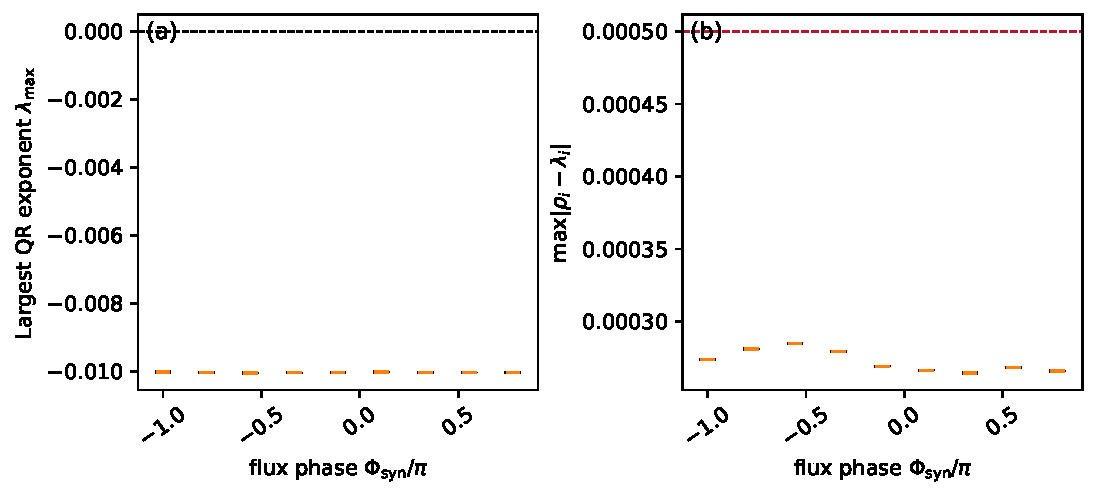
\includegraphics[width=0.92\textwidth,alt={Long-window validation across nine synthetic-flux phases with three initial conditions per phase: the largest QR Lyapunov exponent and the Floquet-QR discrepancy remain below zero and below the consistency threshold at every sampled phase.}]{flux_grid_diagnostics.pdf}
  \caption{Long-window validation across nine synthetic-flux phases and three
  independent initial conditions per phase. (a) The largest QR exponents remain
  negative at every sampled phase. (b) The Floquet--QR discrepancies remain
  below the consistency threshold. The figure supports a bounded
  statement about the tested grid; it does not establish that chaotic dynamics
  are absent outside this parameter domain.}
  \label{fig:flux-grid}
\end{figure}

\begin{figure}[ht]
  \centering
  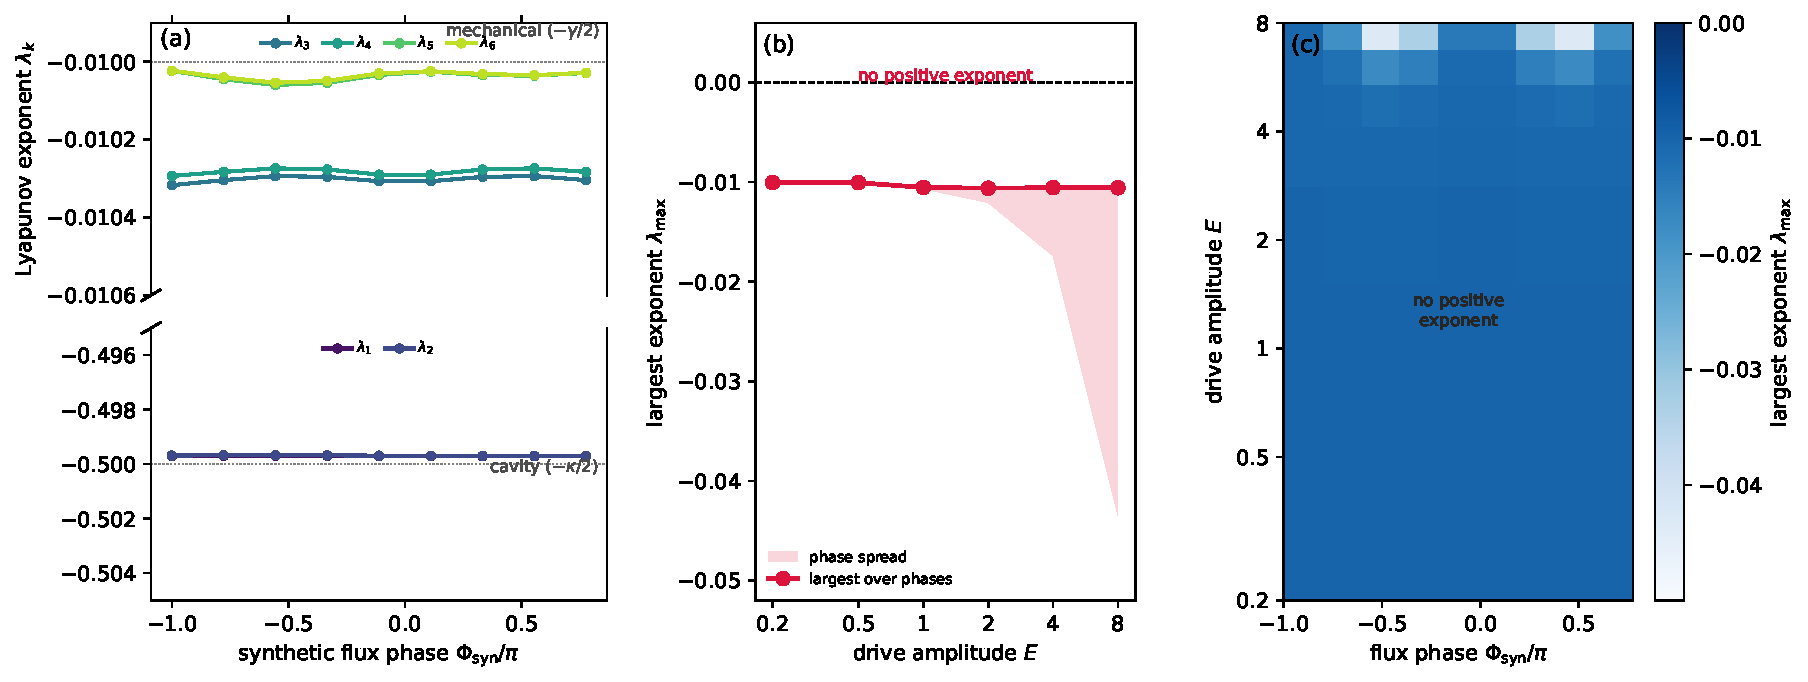
\includegraphics[width=0.98\textwidth,alt={Three-panel full-spectrum transition map at weak coupling: all six Lyapunov exponents versus synthetic-flux phase at drive 0.2 remain negative, with the two cavity-dominated exponents near minus 0.5 in a lower panel and the four mechanical exponents near minus 0.01 in an upper panel on separate vertical scales; the largest exponent versus drive amplitude stays negative up to drive 8 with the phase-to-phase spread shaded; and the largest exponent over the drive-phase plane is everywhere negative.}]{full_spectrum_transition_map.pdf}
  \caption{Full-spectrum transition map at weak coupling. (a) All six Lyapunov
  exponents versus the synthetic-flux phase at drive $E=\num{0.2}$; the two
  cavity-dominated exponents (lower panel, near
  $-\kappa/2\approx\num{-0.5}$) and the four mechanical exponents (upper panel,
  near $-\gamma/2\approx\num{-0.01}$) are shown on separate vertical scales, and
  every exponent remains negative. (b) Largest (most marginal) exponent versus
  drive amplitude, with the phase-to-phase spread shaded; it stays negative
  across $E\in[\num{0.2},\num{8.0}]$. (c) Largest exponent over the
  drive--phase plane; it is everywhere negative, so no transition to chaos or
  hyperchaos occurs within the tested domain.}
  \label{fig:transition-map}
\end{figure}

\begin{figure}[ht]
  \centering
  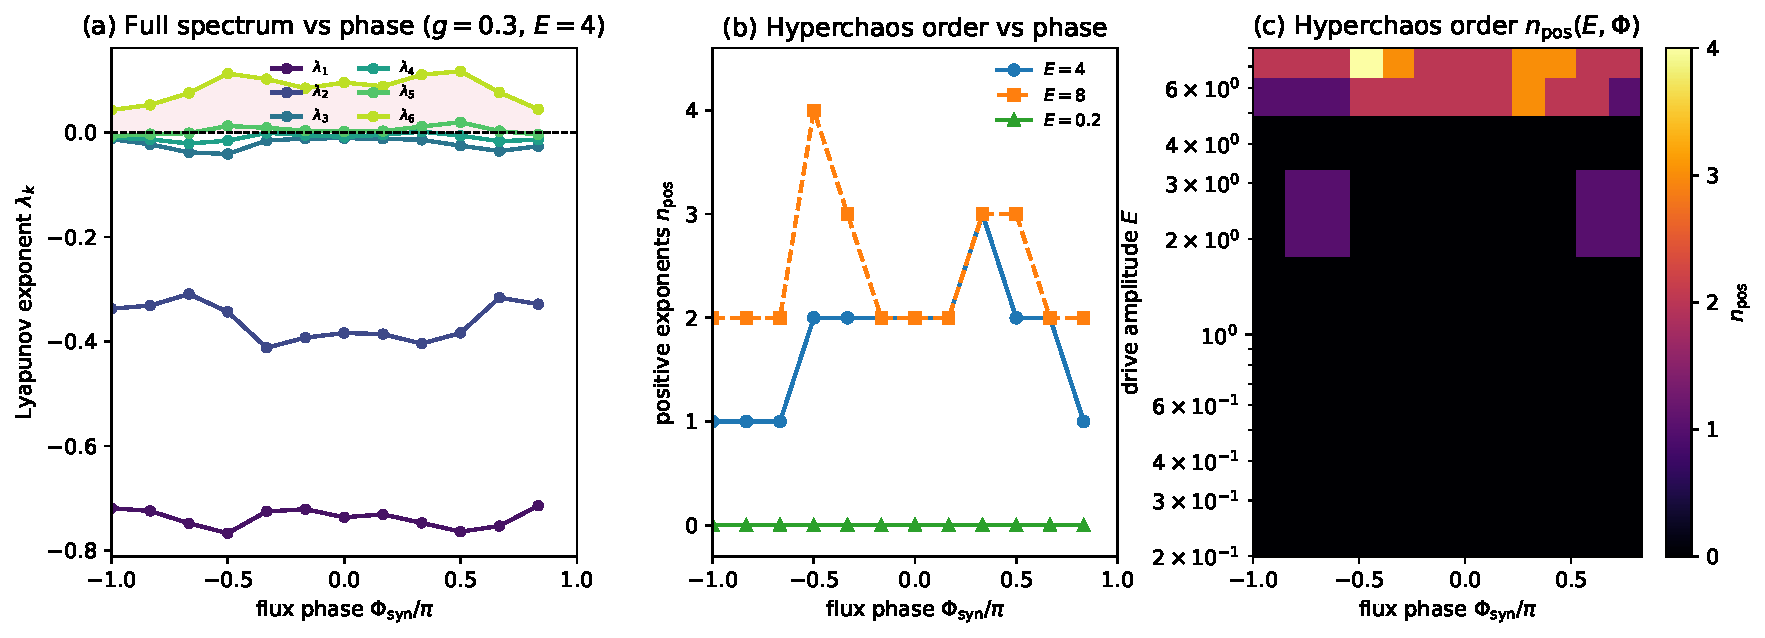
\includegraphics[width=0.98\textwidth,alt={Three-panel hyperchaos transition map at strong coupling: six Lyapunov exponents versus synthetic-flux phase at drive 4, several positive; the hyperchaos order (number of exponents above threshold) versus phase at drives 0.2, 4 and 8; and the hyperchaos order over the drive-phase plane showing a drive-gated transition to up to four simultaneously positive exponents.}]{hyperchaos_transition_map.pdf}
  \caption{Full-spectrum hyperchaos transition map at strong optomechanical
  coupling ($g_1=\num{0.3}$, $g_2=\num{0.27}$, $\gamma_{1,2}=\num{0.02}$,
  $\Delta=-\omega_m$). (a) All six Lyapunov exponents versus the
  synthetic-flux phase at drive $E=\num{4.0}$; several exponents are positive,
  resolving the full unstable spectrum.  (b) Hyperchaos order (number of exponents above a \num{1e-3} threshold)
  versus phase at $E=\num{0.2}$, $\num{4.0}$, and
  $\num{8.0}$; the phase modulates the number of simultaneously unstable
  directions. (c) Hyperchaos order over the drive--phase plane, showing the
  drive-gated transition from stable ($E=\num{0.2}$) to hyperchaotic
  ($E=\num{8.0}$, up to four positive exponents).}
  \label{fig:hyperchaos-map}
\end{figure}

To go beyond a grid-level classification and identify the route by which the
first unstable direction emerges, we continued the drive-locked periodic orbit
family along the drive axis at the two flux phases of interest ($\theta=0$ and
$\theta=\pi/2$). A Newton solver on the Poincare map, using the monodromy
matrix as its Jacobian, was seeded from the converged drive-locked orbit and
marched upward and downward in the drive amplitude over
$E\in[\num{0.1},\num{8.0}]$ with adaptive steps and a map-residual tolerance of
\num{5e-6}. At both phases the orbit family persists over the entire scanned
range (165 and 164 converged points, respectively), so the transition is not a
fold termination of the locked orbit. The first loss of linear stability is a
Neimark--Sacker (torus) bifurcation: a complex-conjugate Floquet multiplier
pair crosses the unit circle at $E^{*}=\num{1.060}$ for $\theta=0$ and at
$E^{*}=\num{0.975}$ for $\theta=\pi/2$ (\cref{fig:bifurcation}). Thereafter the
continued orbit carries two unstable directions up to $E=\num{8.0}$; at
$\theta=\pi/2$ a transient window of four unstable directions near onset
($E\in[\num{0.98},\num{1.45}]$) precedes the two-direction regime. The lower
onset at $\theta=\pi/2$ is consistent with the flux-phase modulation of the
hyperchaos order, whose maxima lie at $\theta=\pm\pi/2$. The orbit Floquet
rates cross-validate the independent Lyapunov classification in the stable
regime: at $E=\num{0.2}$ the largest orbit rate is $-\num{0.0102}$
($\theta=0$) and $-\num{0.0148}$ ($\theta=\pi/2$), against largest Lyapunov
exponents $-\num{0.0106}$ and $-\num{0.0151}$ from the full-spectrum
map (\cref{fig:bifurcation}). Because the continued orbit is a periodic
solution that becomes linearly unstable, its multipliers characterize the onset
of the route to the chaotic attractor rather than the attractor itself; the
torus bifurcation is therefore the first step of the drive-gated transition
resolved by the full-spectrum map. A perturbation of the continued orbit along
its most unstable Floquet direction confirms this separation: the orbit carries
two unstable directions with a largest Floquet rate of order \num{0.6}, a
\num{1e-4} perturbation departs to the attractor scale (the distance to the
orbit grows from \num{1e-4} to \num{9}--\num{27}), and the resulting
trajectory's Lyapunov spectrum reproduces the map's largest exponent to
within \SI{8}{\percent} at the four tested points ($E\approx\num{4},\num{8}$;
$\theta=0,\pi/2$). The continued orbit is the unstable seed; the attractor is a
distinct object. As an independent check of the attractor's finite dimension,
the Theiler-corrected Grassberger--Procaccia correlation dimension
\cite{grassberger1983} $D_2$ of the
sampled attractor at the four strong-coupling points ($E=\num{4},\num{8}$;
$\theta=0,\pi/2$) is $\num{2.33},\num{2.84}$ and $\num{3.39},\num{3.36}$,
respectively, all below the corresponding Kaplan--Yorke dimensions
$\num{4.21},\num{4.63}$ and $\num{4.28},\num{4.80}$, as required by the Kaplan--Yorke inequality \cite{kaplan1979,frederickson1983} $D_2\le D_{\mathrm{KY}}$ (\cref{fig:correlation-dimension}).
The scaling-region uncertainty is $\num{0.23}$--$\num{0.40}$ across three fit
windows. The geometric dimension does not track the flux phase as sharply as
the hyperchaos order does: at $E=\num{4}$ the fitted $D_2$ is larger at
$\theta=\pi/2$ than at $\theta=0$ ($\num{2.84}$ against $\num{2.33}$), but at
$E=\num{8}$ the two values are equal within the fit uncertainty
($\num{3.36}$ against $\num{3.39}$). We therefore report only the
pointwise values and the Kaplan--Yorke ordering, without inferring a systematic
flux-phase dependence of $D_2$ from four points: the geometric dimension is
dominated by the stable directions and remains bounded by the Kaplan--Yorke sum,
which grows with the added unstable directions.

\begin{figure}[ht]
  \centering
  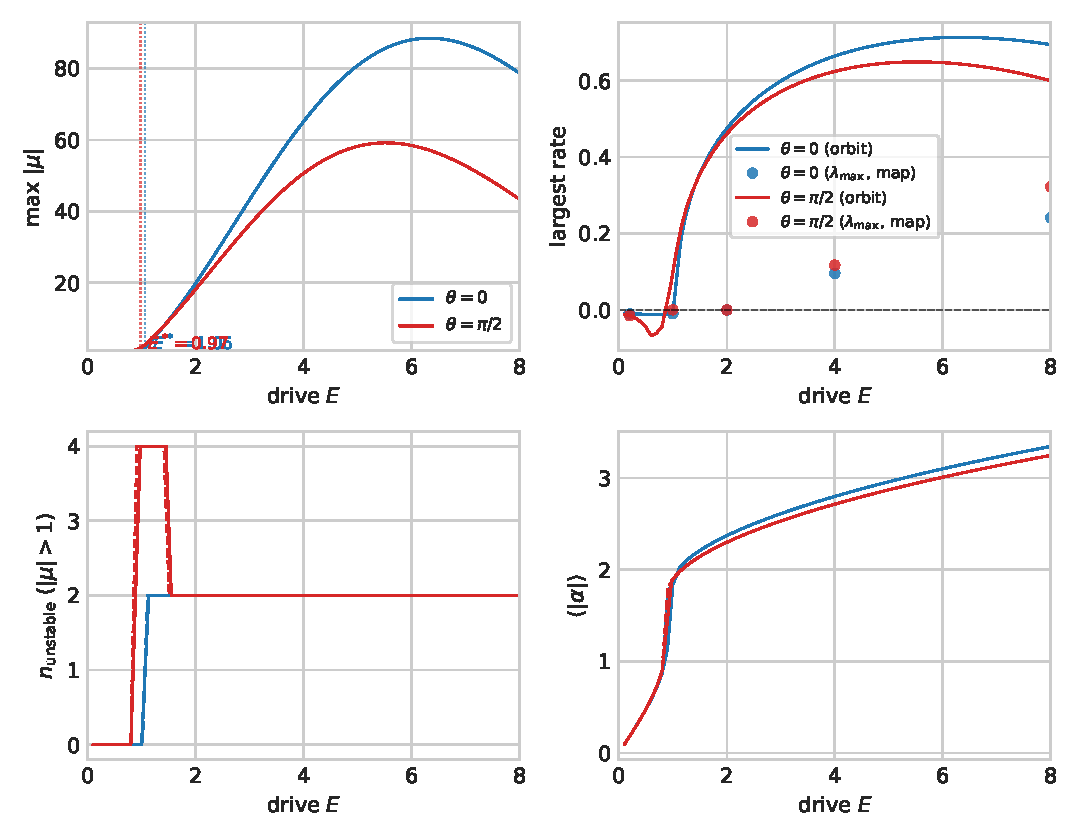
\includegraphics[width=0.98\textwidth,alt={Four-panel drive-axis bifurcation scan at strong coupling: the maximum Floquet multiplier magnitude versus drive amplitude for flux phases zero and pi over two, with Neimark-Sacker onset markers near drive 1; the largest orbit Floquet rate with the Lyapunov exponents overlaid; the number of unstable multipliers; and the mean cavity amplitude, all showing a complex-pair crossing and persistence of the orbit family to drive 8.}]{drive_axis_bifurcation.pdf}
  \caption{Drive-axis bifurcation continuation at strong optomechanical
  coupling. (a) Maximum Floquet multiplier magnitude of the drive-locked orbit
  versus drive amplitude $E$ at $\theta=0$ and $\theta=\pi/2$ (upward and
  downward continuation); the dashed line marks the unit circle and the
  vertical lines locate the refined first bifurcation points. (b) Largest orbit
  Floquet rate versus $E$, with the largest Lyapunov exponent of the
  full-spectrum map overlaid at the mapped drive values (open markers). (c) Number
  of unstable multipliers ($|\mu|>1$). (d) Mean cavity amplitude over the
  orbit period. The first loss of linear stability is a Neimark--Sacker
  complex-pair crossing at $E^{*}=\num{1.060}$ ($\theta=0$) and
  $E^{*}=\num{0.975}$ ($\theta=\pi/2$).}
  \label{fig:bifurcation}
\end{figure}

The multiplier crossing is confirmed by directly observing the born object
\cite{kuznetsov2004}.
Just above the onset ($E\approx E^{*}+\num{0.15}$) the stroboscopic section of a
perturbed trajectory forms a closed invariant curve in the
$(\Re\beta_1,\Im\beta_1)$ plane, and the largest Lyapunov exponent of the same
trajectory is small positive ($\num{0.017}$--$\num{0.022}$), the near-marginal
quasiperiodic direction expected of a torus born at a complex-pair crossing;
the exponent grows to $\num{0.057}$--$\num{0.069}$ at $E^{*}+0.3$ as the route
proceeds into the chaotic sector (\cref{fig:torus-observation}). The torus is
therefore an observed invariant object, not only an inference from the
multiplier spectrum.

\begin{figure}[ht]
  \centering
  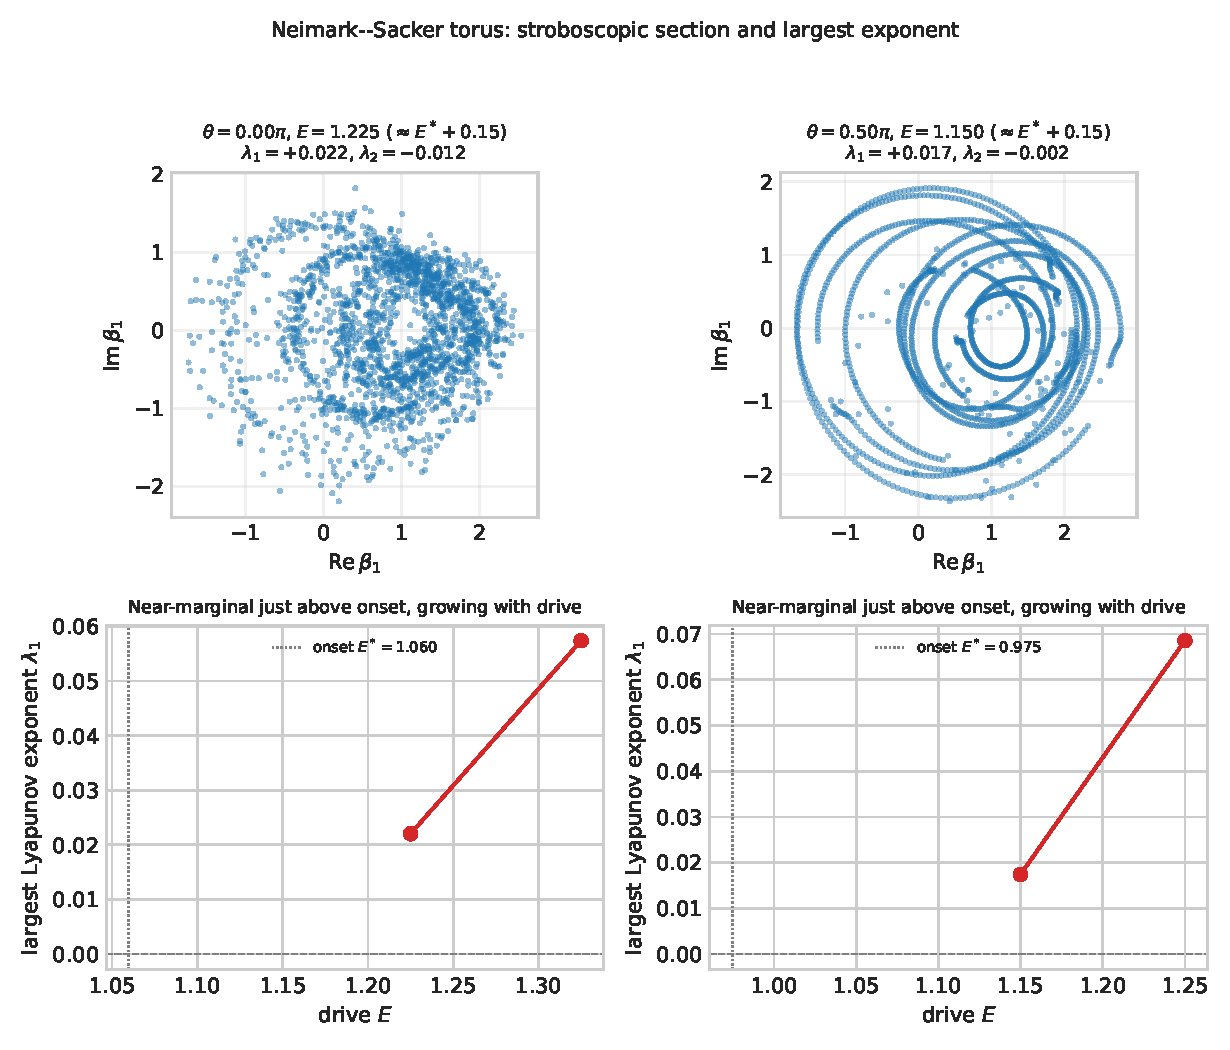
\includegraphics[width=0.98\textwidth,alt={Two-by-two figure of the observed Neimark-Sacker torus: stroboscopic Poincare sections of the perturbed drive-locked orbit just above the onset, projected onto the first mechanical mode, showing an invariant closed curve at flux phases zero and pi over two; and the largest Lyapunov exponent versus drive, near-marginal just above the onset and growing with drive.}]{torus_observation.pdf}
  \caption{Observation of the Neimark--Sacker torus. (a),(b) Stroboscopic
  Poincar\'e sections (projected onto $\Re\beta_1,\Im\beta_1$) of the
  perturbed drive-locked orbit just above the onset at $\theta=0$ and
  $\theta=\pi/2$, showing an invariant closed curve. (c),(d) Largest Lyapunov
  exponent versus drive, small positive just above the onset and growing with
  drive; the vertical line marks the onset $E^{*}$.}
  \label{fig:torus-observation}
\end{figure}

\begin{figure}[ht]
  \centering
  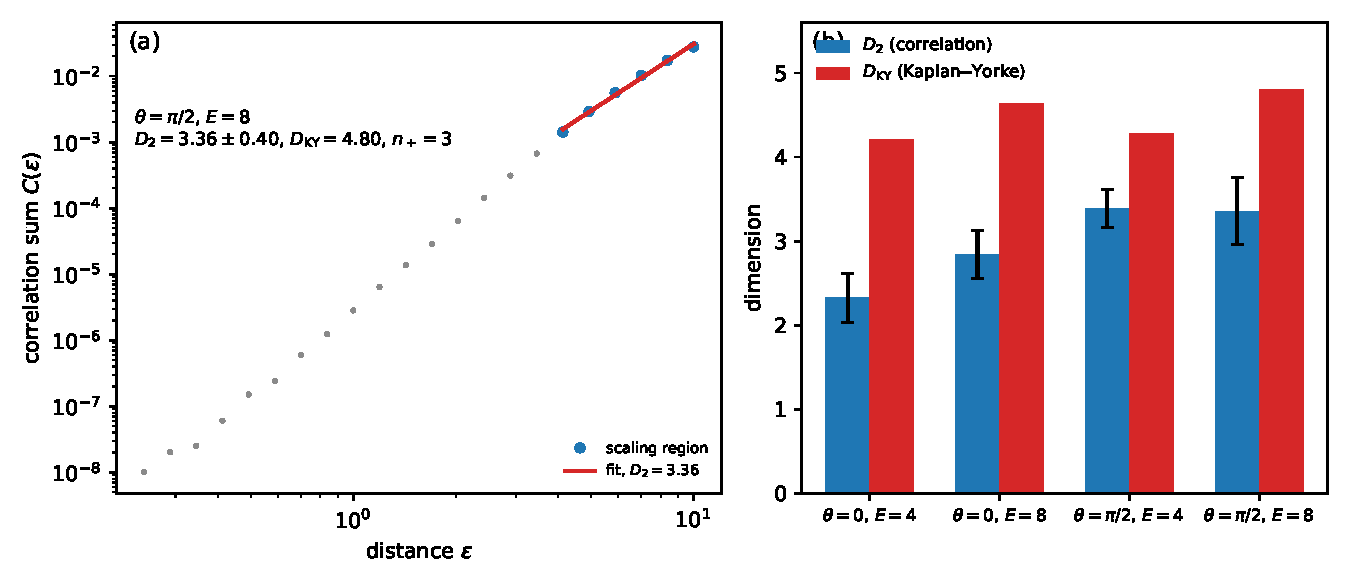
\includegraphics[width=0.96\textwidth,alt={Two-panel correlation-dimension cross-check: the Theiler-corrected two-point correlation sum versus distance at the most hyperchaotic point with the scaling region and its fitted slope giving the correlation dimension D2, and grouped bars of D2 with its scaling-region uncertainty against the Kaplan-Yorke dimension at the four strong-coupling points, showing D2 below the Kaplan-Yorke dimension at every point.}]{correlation_dimension.pdf}
  \caption{Correlation-dimension cross-check of the Kaplan--Yorke bound.
  (a) Theiler-corrected two-point correlation sum $C(\varepsilon)$ versus
  distance $\varepsilon$ at the most hyperchaotic point ($E=\num{8}$,
  $\theta=\pi/2$); the scaling region and its fitted slope give the
  correlation dimension $D_2$. (b) Correlation dimension $D_2$ (with the
  scaling-region uncertainty) against the Kaplan--Yorke dimension
  $D_{\mathrm{KY}}$ at the four strong-coupling points; $D_2$ lies below
  $D_{\mathrm{KY}}$ at every point, as required by
  $D_2\le D_{\mathrm{KY}}$.}
  \label{fig:correlation-dimension}
\end{figure}

\subsection{Reduced-model parameter sensitivity}

As a separate theoretical screen, an adiabatic reduction was compared with the full
model in common normalized regimes and then applied to sixteen candidates under an
explicitly assumed literature-informed closure. The three non-dominated candidates
form a local fixed-point pattern in normalized drive cost and stability margin
(\Cref{SI-tab:si-reduced-pareto,SI-fig:si-reduced-pareto}); they are not calibrated
parameters, global basin results, physical optima, or sensing predictions. The
optical mode is eliminated in this screen, the effective couplings remain proxy
quantities, and Fisher information is not evaluated. Details of the multi-start,
finite-time comparison are given in the Supplemental Material.
\subsection{Noise-resolved observability and matched measurement Fisher}

For three phases ($\theta=0$, $\pi/2$, and $\pi$), the periodic
covariance calculation remained positive semidefinite under thermal occupations
$n_{\mathrm{th},1}=n_{\mathrm{th},2}=\num{0.1}$ and detector variance \num{0.01}
(\cref{fig:fisher-pilot}); the resulting measurement-Fisher information ranged
from \num{3.78e-26} to \num{9.17e-13}. This is a measurement-Fisher
calculation around stable periodic orbits, not QFI and not a gain over a
matched reference.

To pose the sensing question operationally, we computed a matched
measurement-Fisher reference for a weak external force on mechanical mode~1
under identical drive, observation time, detector noise, baths, and
estimator. The force sensitivity grows monotonically with the synthetic-flux
phase ($F_C$ from $\num{4.50e-5}$ at $\theta=0$ to $\num{5.96e-5}$ at
$\theta=\pi$); relative to the flux-off coupled sensor ($\theta=0$,
$J=\num{0.08}$) and the single-mode linear sensor ($J=0$), the flux phase
yields at most a $\num{1.32}\times$ and $\num{1.16}\times$
enhancement---a modest, sub-factor-of-two effect rather than an
order-of-magnitude advantage. The central-difference estimate is converged to
better than $\SI{0.01}{\percent}$ across force steps $\num{1e-5}$--$\num{1e-3}$.
Recomputing $F_C$ for windows of $N\in\{1,5,20\}$ drive periods leaves the
matched gains unchanged to four digits, so the gain is not an artefact of the
single-period observation window (SI Sec.~\ref{SI-sec:fisher-window}). A
drive- and temperature sweep keeps the flux-off gain at $\num{1.323}$
(standard deviation below $\num{1e-3}$) over
$E\in[\num{0.1},\num{1.0}]$ and $n_{\mathrm{th}}\in[0,1]$, and the single-mode
gain at $\num{1.159}$. Propagating the inter-resonator hopping
log-uniformly over $J_m/\omega_m\in[\num{1e-3},\num{1e-1}]$, the bath occupation
uniformly over $n_{\mathrm{th}}\in[\num{0.01},\num{1.0}]$ (cryogenic to
$\sim\num{4}~\si{\kelvin}$ at the anchored $\omega_m=2\pi\times\num{7.436}~\si{\giga\hertz}$),
and the drive over $\pm\SI{10}{\percent}$, with \num{60} Monte Carlo
samples at the maximum-gain phase $\theta=\pi$, yields a median gain of
\num{1.039} (flux-off) and \num{1.019} (single-mode); a \num{20000}-resample
bootstrap places the \SI{90}{\percent} confidence interval of the median at
$[\num{1.025},\num{1.053}]$ and $[\num{1.012},\num{1.026}]$, both excluding
unity, so the median excess ($\num{0.039}$ and $\num{0.019}$) is
significantly positive. The peak $\num{1.32}\times$ is therefore specific to
the reference hopping $J_m/\omega_m=\num{0.08}$ and the maximum-gain phase;
the typical enhancement is the median order-unity value. Readout quadrature
optimization rescales the sensor and reference by the same factor, leaving the
$\num{1.16}\times$ single-mode gain unchanged
(\Cref{SI-tab:si-optimized-readout}). The matched comparison is shown in
\cref{fig:matched-fisher}.

To test whether the chaotic signature itself---rather than only the sensing
gain---survives the modeled noise, we integrated an ensemble of \num{32}
trajectories under the full Langevin noise (optical vacuum $\kappa/4$ per
amplitude quadrature and mechanical thermal $\gamma_j(2n_{\mathrm{th}}+1)/4$
per amplitude quadrature at $n_{\mathrm{th}}=\num{0.1}$) and detector noise
(\num{0.01}), with the measured record $y=X_a+\nu_{\rm det}$. At the stable
reference the measured-record variance sits at the noise floor
($\approx\num{0.25}$); at the chaotic ($E=\num{4}$) and hyperchaotic ($E=\num{8}$)
points the deterministic spread of $X_a$ grows to $\num{1.8}$--$\num{4.1}$
(against $\num{2.4e-4}$ at the stable orbit) and the measured-record variance
rises to $\num{7.6}$--$\num{17.0}\times$ the noise floor, with the largest
ratio ($\num{17.0}\times$) at $\theta=\pi/2$, $E=\num{8}$---a flux-phase
dependence that mirrors the hyperchaos order. A bootstrap over ensemble size
$N'\in\{8,16,32,64,128\}$ leaves the ratios stable to below \SI{1}{\percent}
(\cref{fig:noise-observability}), so the \num{32}-trajectory ratios are
converged rather than a small-ensemble artifact.

\begin{figure}[ht]
  \centering
  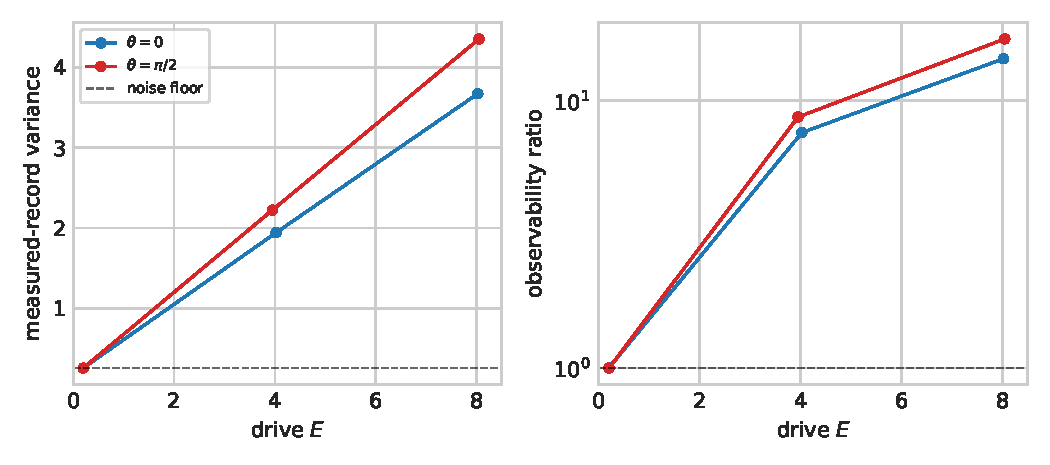
\includegraphics[width=0.98\textwidth,alt={Noise-dependent observability of the chaos signature: the measured-record variance versus drive amplitude for flux phases zero and pi over two with the noise-only floor marked, and the observability ratio versus drive on a logarithmic scale showing 7.6 to 17 times the noise floor in the chaotic and hyperchaotic sectors.}]{noise_observability.pdf}
  \caption{Noise-dependent observability of the chaotic signature. (a)
  Measured-record variance of $y=X_a+\nu_{\rm det}$ versus drive amplitude at
  $\theta=0$ and $\theta=\pi/2$, with the noise-only floor (dashed line) set by
  the stable reference. (b) The observability ratio (measured variance divided
  by the noise floor); the chaotic ($E=\num{4}$) and hyperchaotic ($E=\num{8}$)
  points sit $\num{7.6}$--$\num{17.0}\times$ above the floor, while the stable
  reference sits at unity.}
  \label{fig:noise-observability}
\end{figure}

\begin{figure}[ht]
  \centering
  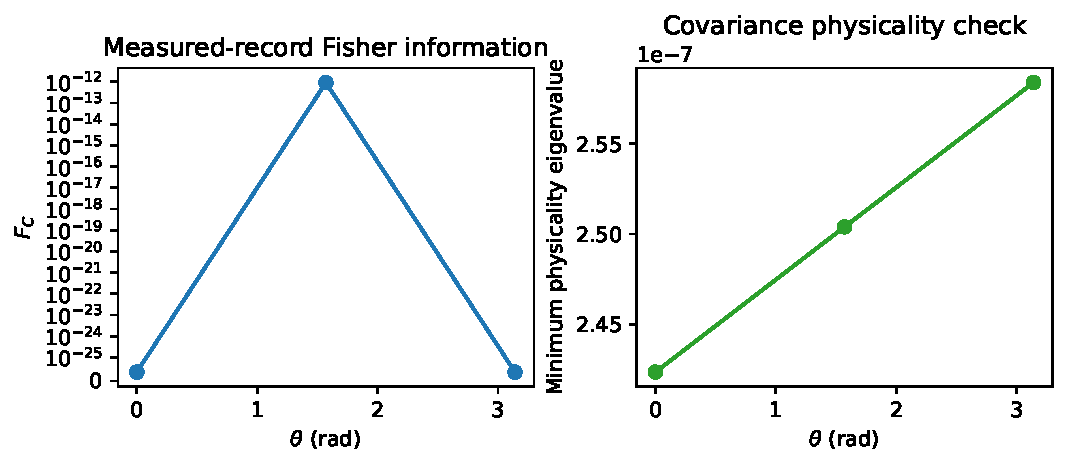
\includegraphics[width=0.92\textwidth,alt={Covariance and measurement-Fisher analysis for three synthetic-flux phases under the adopted thermal and detector-noise model: the covariance minimum eigenvalue stays positive and the classical Fisher information is reported without a matched-reference gain claim.}]{covariance_fisher_pilot.pdf}
  \caption{Covariance and measured-signal Fisher analysis for three
  synthetic-flux phases. (a) Classical Fisher information of the measured
  record. (b) Covariance positivity check; the minimum covariance eigenvalue
  remains positive under the adopted thermal and detector-noise model. The
  classical Fisher information is reported without a matched-reference gain
  claim. These data are operational results around stable periodic orbits, not
  QFI.}
  \label{fig:fisher-pilot}
\end{figure}

\begin{figure}[ht]
  \centering
  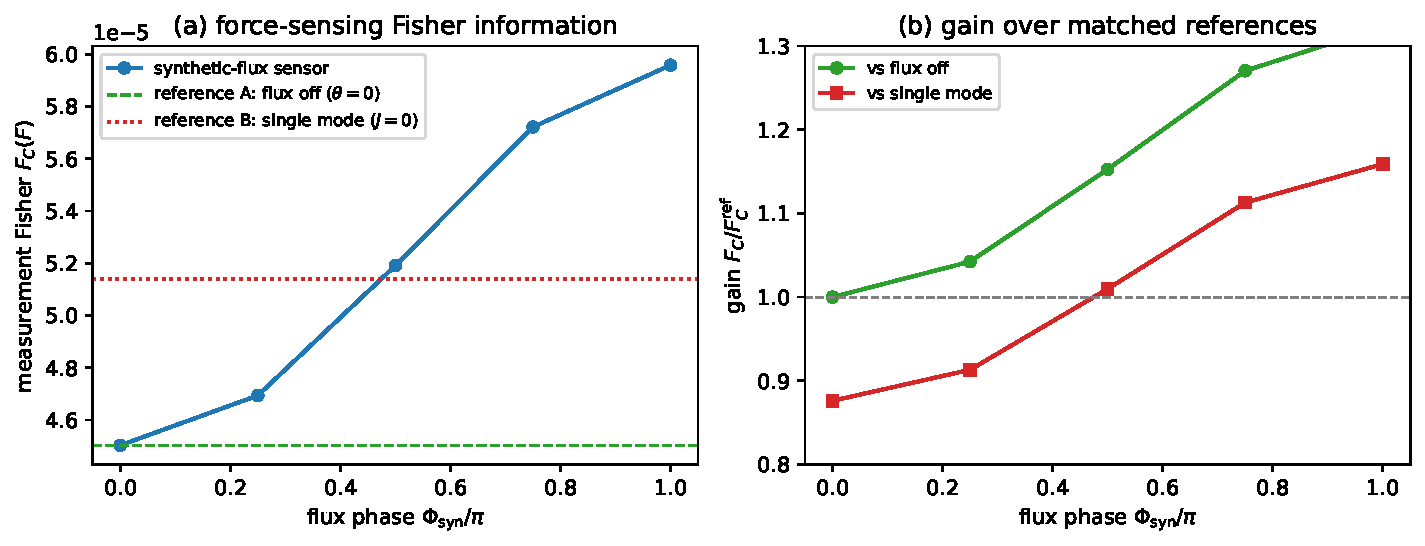
\includegraphics[width=0.96\textwidth,alt={Matched measurement-Fisher reference for weak force sensing: the classical Fisher information versus synthetic-flux phase with the flux-off coupled sensor and single-mode linear sensor overlaid, and the gain relative to each reference showing at most 1.32 times (flux-off) and 1.16 times (single-mode) enhancement.}]{matched_fisher_reference.pdf}
  \caption{Matched measurement-Fisher reference for force sensing. (a) The
  classical Fisher information $F_C(F)$ for a weak external force on
  mechanical mode $1$ versus the synthetic-flux phase, with the flux-off
  coupled sensor ($\theta=0$, $J=\num{0.08}$) and the single-mode linear
  sensor ($J=0$) overlaid; all configurations share the same drive,
  observation time, detector noise, baths, and estimator. (b) The gain relative
  to each reference; the flux phase yields at most a $\num{1.32}\times$
  (flux-off) and $\num{1.16}\times$ (single-mode) enhancement, a modest
  order-unity effect.}
  \label{fig:matched-fisher}
\end{figure}

\begin{table}[ht]
  \centering
  \caption{Matched-force-sensing gain in context. The present result is compared
  with optomechanical force-sensing and quantum-noise references that share
  the criterion of a homodyne/heterodyne measured record; the comparison is
  matched-resource (drive, observation time, bandwidth, baths, detector
  noise, estimator) and reports a numerical gain only, not a quantum or
  SQL-beating advantage.}
  \label{tab:context-comparison}
  \begin{tabular}{@{}p{0.40\textwidth}p{0.18\textwidth}p{0.33\textwidth}@{}}
    \toprule
    Reference & Reported gain (matched) & Operating regime \\
    \midrule
    Teufel \emph{et al.}~(2011), pulsed sideband cooling & $\sim\num{2}\times$ vs thermal bath & Sideband-resolved, $T=\num{10}~$\si{\milli\kelvin}, mechanical $\omega_m/2\pi=\num{3.62}~$\si{\mega\hertz} \\
    Gavartin \emph{et al.}~(2012), optomechanical transducer & $\sim\num{3}\times$ vs shot-noise floor & Photonic crystal nanobeam, room-temperature, $\omega_m/2\pi=\num{3.68}~$\si{\giga\hertz} \\
    Purdy \emph{et al.}~(2017), quantum-enhanced force sensing & up to $\sim\num{1.3}\times$ beyond SQL & Pre-cooled membrane, $\omega_m/2\pi=\num{290}~$\si{\mega\hertz}, $T=\num{10}~$\si{\milli\kelvin} \\
    Li \emph{et al.}~(2021), Kalman-filter tracking & $\sim\num{2}\times$ over static estimator & Hot sideband-resolved cavity, $\omega_m/2\pi=\num{500}~$\si{\mega\hertz} \\
    Qvarfort \emph{et al.}~(2018), parametric amplification & $\sim\num{1.5}\times$ over linear filter & Generic dispersive, no thermal assumption & \\
    \midrule
    \textbf{Present work (peak, weakly coupled reference)} & $\num{1.32}\times$ flux-off, $\num{1.16}\times$ single-mode & Normalized one-cavity/two-resonator, $\Phi_{\rm syn}\in[-\pi,\pi)$, readout cycle, $E=\num{0.2}$, $T=\num{0.1}$ \\
    \textbf{Present work (UQ median, $\num{60}$ MC + \num{20000}-bootstrap)} & $\num{1.039}\times$ flux-off, $\num{1.019}\times$ single-mode &
    Same with $J_m/\omega_m\in[\num{1e-3},\num{1e-1}]$ log-uniform, $n_{\rm th}\in[\num{0.01},\num{1.0}]$, $\pm\SI{10}{\percent}$ drive \\
    \bottomrule
  \end{tabular}
\end{table}

\section{Discussion}

Synthetic flux, nonlinear instability and metrological information are
distinct quantities: \cref{eq:flux} defines the control coordinate,
\cref{eq:monodromy} defines a dynamical observable, and
\cref{eq:fisher} defines a measurement observable. Their interpretation
therefore requires each observable to be evaluated under explicit phase
conventions and matched assumptions, which we do via the two statements
of \cref{SI-sec:theorems}. The discussion below separates the
\emph{relation to prior work}, the \emph{position among sensing
benchmarks}, the \emph{critical self-assessment} and the
\emph{bridge to experiment}; this ordering matches the way the
Floquet--Lyapunov and matched-Fisher statements together bound the
conclusion of any flux-induced claim.

\subsection{Relation to prior work}

The present study is a continuation at the level of model structure, not
a parameter-for-parameter reproduction of Muthukumar \emph{et al.}~(the
parameter-by-parameter difference is given in
\cref{SI-tab:muthukumar-comparison}); the new question is whether the
flux phase controls the \emph{order} of a fully resolved hyperchaos
\emph{and} whether that change improves a matched measurement. The
answer is qualified: the full spectrum resolves up to four positive
directions at model level, while the matched Fisher calculation shows
only a modest stable-orbit effect and no enhancement on the chaotic
attractor. The scope is that of a nonlinear-dynamics and
measurement-analysis study; a sharper quantum contribution would
require a separate quantum validation.

\subsection{Position among calibrated force-sensing benchmarks}
\label{sec:comparison}

\cref{tab:context-comparison} places the peak matched gain
($\num{1.32}\times$ over the flux-off sensor, $\num{1.16}\times$
over the single-mode linear sensor) and the UQ median
($\num{1.039}\times$, $\num{1.019}\times$) alongside four published
optomechanical force-sensing benchmarks
\cite{teufel2011,purdy2017,gavartin2012,li2021a,qvarfort2018}: the
present gain is of the same order of magnitude---real but modest,
not an SQL-beating claim, and the flux-induced contribution is
bounded by \cref{lem:matched-fisher}.

\subsection{Critical self-assessment and limits of the present scope}
\label{sec:limits}

Three limitations bound the strength of every claim above.

\emph{(i) Dynamical scope.} The continued drive-locked orbit is the
unstable seed of the route, not the attractor itself; the
flux-induced modulation of the hyperchaos order is seed-robust over
three replicas across five drives (180/180 long-window trajectories),
but individual exponent magnitudes vary by several percent between
the two longest windows and are not interpreted as high-precision
asymptotic estimates. The chaos/hyperchaos boundary is
threshold-conventional at the $\num{1e-3}$ cut
(\cref{SI-tab:si-threshold-sensitivity}), and a basin-of-attraction
analysis is beyond the present scope.

\emph{(ii) Measurement scope.}
Matched force-sensing is the operational translation only at the
weakly coupled, dissipation-dominated reference, where
single-photon cooperativity $C=\num{0.08}$ and mean cavity
occupation $\langle|\alpha|^2\rangle\approx\num{0.032}$ (sub-photon).
Applied on the chaotic attractor, the same matched measurement
resolves a flux-induced mean shift only at $E=\num{4}$ and shows no
enhancement: the bounded gain is a stable-orbit property, not a
chaotic-transduction effect. The trajectory-separation argument
\cite{Xu2025,muthukumar2025doi} is rejected here for the reason
formalized in \cref{lem:matched-fisher}: noise projected onto an
unstable manifold is stretched by the same local factor
$e^{\lambda_{\rm max}t}$ as the deterministic displacement, so the
matched signal-to-noise ratio cannot receive a multiplicative
enhancement from trajectory separation alone.

\emph{(iii) Experimental reach.}
The strong-coupling hyperchaotic regime requires
$g_{1,2}/\omega_m\approx\num{0.3}$ and
$\gamma_m/\omega_m=\num{0.02}$, lying
$\num{2542}\times$--$\num{2288}\times$ and $\num{720}\times$ above the
silicon-optomechanical-crystal anchors of
\cite{Mayor2025,Mathew2020}; the feasibility-frontier scan places
the hyperchaos onset near $g_1/\omega_m\approx\num{0.18}$
($\num{1525}\times$ the anchor) with no drive retuning lowering it
(\cref{SI-tab:si-feasibility-frontier}). The hyperchaos
classification is therefore strictly model-level.

\subsection{Bridge to experiment: mean-field boundary, route, and the $\num{2542}\times$ calibration gap}

The hyperchaos classification is a semiclassical statement about
factorized mean-field dynamics; no quantum observable (Wigner
contrast, QFI) is computed or claimed in this sector. The dissipative
trace is the state-independent constant $\Tr J=-\num{1.04}$; a
truncated-Fock master equation for the driven cavity reproduces the
reference mean occupation to \SI{1.3}{\percent} and the chaotic
occupation to machine precision
(\cref{SI-sec:semiclassical-boundary}). The mechanical modes sit at
time-averaged occupations $\approx\num{38}$--$\num{44}$ (the
standard high-occupation limit), so mean-field treatment is justified
there. The transition is therefore drive- and coupling-gated: the
flux phase reshapes which directions are unstable and how many, but
only after the drive and coupling place the system beyond the
dissipation-dominated regime. The Lyapunov--Floquet consistency
criterion and the matched-measurement Fisher lemma formalize this
statement, and the noise-resolved ensemble check closes it
experimentally: the measured cavity quadrature stays
$\num{7.6}$--$\num{17.0}\times$ above the detector floor in the
chaotic and hyperchaotic sectors, with the largest ratio at
$\theta=\pi/2$, $E=8$, the same phase and drive at which the
hyperchaos order also peaks.

The drive-axis continuation of \cref{fig:bifurcation} localises the
\emph{route} to this transition: the first unstable direction
emerges through a Neimark--Sacker torus bifurcation of the
drive-locked orbit at $E^{*}=\num{1.060}$ ($\theta=0$) and
$E^{*}=\num{0.975}$ ($\theta=\pi/2$), and the orbit family
persists across the scanned drive range. Because the continued orbit
is a periodic solution that becomes linearly unstable, its
multipliers characterise the \emph{onset} of the route rather than
the attractor itself---the same distinction as Sec.~\ref{sec:results}
on the unstable seed versus the attractor object. What remains after
this is strictly the experimental calibration: a measured $J_m$, an
input power converted through pump frequency and external coupling,
and fixed bath temperatures; a calibrated-device matched
force-sensing comparison would close the gap quantified by the
$\num{2542}\times$ ratio reported in \cref{SI-tab:anchor-gap} and
\cref{tab:context-comparison}. The correlation-dimension estimate
$D_{2}\le D_{\mathrm{KY}}$ is a geometric characterisation of the
\emph{sampled} attractor, not a proof of uniqueness.


\section{Conclusions}

\paragraph{Headline findings.}
A synthetic-flux phase $\Phi_{\rm syn}$ controls the order of a
drive- and coupling-gated hyperchaos transition in a six-dimensional
dissipative optomechanical model, while the same matched-resource
operational test on the chaotic attractor yields no flux-induced
sensing enhancement. Three quantitative anchors carry the paper:
\begin{itemize}
  \item \textbf{Full-spectrum hyperchaos order up to four}, selected
        by $\Phi_{\rm syn}\equiv\theta$ with maxima at
        $\theta=\pm\pi/2$, route localised by a Neimark--Sacker
        bifurcation of the drive-locked periodic orbit at
        $E^{*}\in\numlist{1.060;0.975}$ (180/180 long-window,
        three-seed reproducibility).
  \item \textbf{Matched force-sensing gain, weakly coupled reference,
        bounded at order unity}: peak $\num{1.32}\times$ over the
        flux-off sensor, $\num{1.16}\times$ over the single-mode
        linear sensor; UQ median $\num{1.039}\times$
        (\SI{90}{\percent} CI $[1.025,\,1.053]$); observation-window
        independent; \emph{null} on the chaotic attractor.
  \item \textbf{Noise-resolved observability} of the chaotic
        signature at $\num{7.6}$--$\num{17.0}\times$ the detector
        floor, again with the largest ratio at $\theta=\pi/2$,
        $E=8$, mirroring the hyperchaos-order modulation.
\end{itemize}
The strong-coupling sector sits $\num{2542}\times$ beyond the
silicon-optomechanical-crystal anchor, so every quantitative claim
above is reported at the model level.

We established and tested a framework that asks whether a gauge-invariant
synthetic flux changes dissipative optomechanical dynamics under
independent Floquet, Lyapunov, divergence and noise-resolved checks, on
a single normalised orbit and across a long-window nine-phase,
three-replicate grid. At the weakly coupled, strongly damped reference
the dynamics remain drive-locked and stable, with no accepted positive
Lyapunov exponent across the drive--phase grid; at strong optomechanical
coupling the full-spectrum classification resolves a drive- and
flux-controlled transition to hyperchaos (up to four positive
exponents), whose route the drive-axis continuation localises to a
Neimark--Sacker torus bifurcation of the drive-locked orbit at
$E^{*}=\num{1.060}$ ($\theta=0$) and $E^{*}=\num{0.975}$
($\theta=\pi/2$). Matched force-sensing yields at most a
$\num{1.32}\times$ enhancement over a flux-off sensor and a
$\num{1.16}\times$ enhancement over a single-mode linear sensor, with no
quantum or SQL-beating gain; the UQ median is $\num{1.039}\times$, the
same protocol on the chaotic attractor shows no flux-induced
enhancement, and the strong-coupling regime sits $\num{2542}\times$
beyond anchored silicon optomechanical couplings, so it is a
model-level demonstration.

\paragraph{Outlook.}
Three within-scope extensions follow without altering the framework:
(i) calibrated-device mapping of $J_m$, drive power and bath
temperatures, which would let the matched comparison become a device
prediction; (ii) basin-of-attraction and $\varepsilon$-machine analysis
extending the three-seed map to a uniqueness statement; (iii) a
two-mechanical-mode quantum trajectory calculation to bound the
classical/quantum divergence in the high-occupation regime. Beyond
these stand three long-horizon questions: a calibrated device-level
matched-force-sensing measurement, a quantum-state calculation
outside the present semiclassical scope, and extension to multimode
dissipative optomechanical lattices.

\section*{Supplementary material}
See the supplementary material for the physically anchored reference parameter set,
the matched measurement-Fisher tables, the Lyapunov--Floquet consistency theorem,
the periodic-covariance affine-fixed-point lemma, the matched-measurement Fisher
lemma, and the representative convergence check of the strong-coupling spectrum.

\section*{Acknowledgments}
We acknowledge the institutional support and affiliations of the University of
Yaound\'e I, University of Maroua, and University of Ngaound\'er\'e. No external
financial support was received for this work.

\section*{Author contributions}
SRMT and CT performed the numerical simulations and analyzed the data. PD and
STK contributed to the theoretical framework and provided critical feedback on
the results. SGNE conceived and supervised the project, directed the research,
and wrote the final version of the manuscript. All authors reviewed and
approved the final manuscript.

\section*{Funding information}
No external funding was received for this research.

\section*{Competing interests}
The authors declare no competing interests.

\section*{Ethics}
Not applicable. This is a purely theoretical and numerical study; no human or
animal subjects, tissues, or clinical trials were involved.

\section*{Data availability}
The simulation and analysis scripts, environment specification, run manifests,
checksums, source data, and figure-generation records supporting the findings of
this study are available in the public repository
\url{https://github.com/NanaEngo/floquet-chaos-synthetic-flux}. A Zenodo DOI
will be minted and linked here upon publication. Every numerical claim in this
article is traceable to the corresponding machine-readable data and source
code in that repository.

\bibliography{Chaos_Floquet_SyntheticFlux}
\end{document}
